\section{Introduction}
\label{sec:introduction}

Robotic manipulation of dough and other elasto-plastic materials is difficult because an action changes both the visible geometry and the latent mechanical state. This complicates bimanual shaping with tools: a controller must reason about large deformation, contact, rate dependence, and deformation that does not recover after unloading. Data-driven approaches can learn such behaviour from demonstrations or interaction data, but collecting broad physical datasets with robots is expensive. A calibrated simulator could instead generate controlled synthetic trajectories and support model-based action selection, provided that its predictions are tied to measurements of the real material.

This work develops TaichiDough, a real-to-sim pipeline intended for future bimanual dough shaping with two robot-held spatulas. A calibrated RGB-D camera records the dough while motion capture provides the poses of both tools. The initial visible shape is reconstructed into a volumetric particle model, measured tool motion is replayed in a three-dimensional Material Point Method (MPM) simulator, and material parameters are adjusted to reduce disagreement between rendered and recorded depth observations. The same forward model supports a derivative-free Young's-modulus search and checkpointed reverse-mode differentiation through complete trajectories.

The central question is deliberately narrower than camera-based rheometry: what \emph{effective simulator parameters} can one calibrated view and known tool motion constrain? Absolute camera scale does not remove ambiguity among hidden volume, mass, contact, constitutive response, and numerical discretization. We therefore report parameter estimates only for the declared model and setup, and separate training loss from a frozen full-resolution evaluation. The robot execution and synthetic-data learning experiments are future work; the present study establishes and examines the identification pipeline that they require.

\begin{figure*}[t]
    \centering
    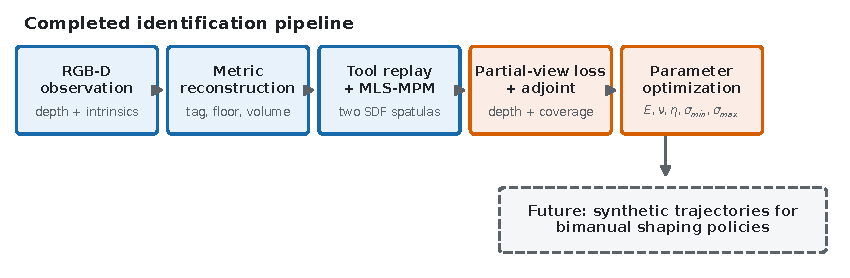
\includegraphics[width=0.98\textwidth]{figures/pipeline_overview.pdf}
    \caption{TaichiDough pipeline. A single calibrated RGB-D camera and recorded poses of two spatulas provide the initial geometry, observations, and boundary motion. A corrected MLS-MPM rollout is projected into the camera and compared with measured depth. Robot execution and synthetic-data learning are intended downstream uses rather than experiments reported here.}
    \label{fig:pipeline}
\end{figure*}

The contributions are:
\begin{itemize}
    \item a metric single-camera pipeline that combines floor-aware volumetric initialization with synchronized replay of two measured spatula trajectories;
    \item a differentiable MLS-MPM formulation for partial depth observations, including bounded optimizer coordinates for elastic, viscous, and principal-stretch parameters; and
    \item a case study using derivative-free and differentiable fitting evidence from recorded dough, including the numerical and identifiability limits that prevent interpreting the current estimates as universal material constants. The runs are not a matched optimizer comparison.
\end{itemize}

\section{Related Work}
\label{sec:related}

\textbf{Deformable simulation and differentiable physics.}
MPM combines Lagrangian material points with an Eulerian grid and is well suited to large deformation and changing topology~\cite{jiang2016mpm}. APIC and MLS-MPM improve particle--grid transfer and provide practical coupling to rigid bodies~\cite{jiang2015apic,hu2018mlsmpm}; singular-value projection has been used to model elasto-plastic yield in graphics materials~\cite{stomakhin2013snow}. Taichi provides the data-oriented programming system used here~\cite{hu2019taichi}. Differentiable simulators such as ChainQueen and DiffTaichi propagate trajectory gradients for control and parameter optimization~\cite{hu2019chainqueen,hu2020difftaichi}, while PlasticineLab applies differentiable physics to soft-body manipulation~\cite{huang2021plasticinelab}. Our contribution is not a new MPM discretization; it connects a corrected MLS-MPM implementation to calibrated partial observations and measured dual-tool motion.

\textbf{Visual real-to-sim identification.}
Prior work estimates deformable-object parameters from images, depth, or point clouds. DiffCloud differentiates point-cloud agreement, and Differentiable Depth calibrates soft-body simulations from a single depth camera~\cite{sundaresan2022diffcloud,arnavaz2023diffdepth}. DPSI studies differentiable physics-based identification for robotic manipulation of elasto-plastic materials~\cite{yang2025dpsi}; EMPM combines differentiable MPM with multi-view RGB-D observations and interaction~\cite{chen2026empm}. These systems demonstrate that visual inverse simulation is established. TaichiDough instead studies a constrained setting with one calibrated RGB-D viewpoint, known two-tool trajectories, reconstructed hidden volume, and a visible-geometry objective. This setting makes nuisance parameters and practical identifiability central: visually similar trajectories can result from different combinations of material, contact, mass, and reconstruction assumptions~\cite{raue2011identifiability,brynjarsdottir2014discrepancy}.

\textbf{Robotic shaping and dough mechanics.}
RoboCraft and RoboCook learn predictive models for shaping elasto-plastic objects with diverse tools~\cite{shi2022robocraft,shi2023robocook}; DoughNet focuses on visual prediction for topological dough manipulation~\cite{bauer2024doughnet}. These works motivate synthetic data and predictive models for bimanual shaping, but do not remove the need to connect a simulator to a particular physical preparation. Food-engineering studies identify dough rheology with controlled loading and force-related measurements. Fabbri and Cevoli, for example, invert a finite-element extrusion model and compare the estimates with capillary rheometry~\cite{fabbri2015dough}. Dough response also depends on formulation, rate, preparation history, and adhesion~\cite{yazar2023doughreview,ghorbel2014adhesion}. Consequently, the Young's modulus, viscosity, and stretch limits fitted here describe the selected constitutive and contact model over the recorded motion; they are not claimed as complete rheological properties of dough.
